\documentclass{article}
\usepackage{graphicx} % Required for inserting images
\usepackage[top=0.5in, bottom=0.8in, left=0.8in, right=0.8in]{geometry} % Adjust margin size here
\usepackage{graphicx} % Required for inserting images


\title{Sequential Recommendation }
\author{Alokam Gnaneswara Sai}
\date{}

\begin{document}

\maketitle


\section{Objective}
\begin{table}[h!]
\centering
\caption{Symbol Definitions}
\begin{tabular}{|c|l|}
\hline
\textbf{Symbol} & \textbf{Definition} \\ \hline
$|U| = n$ & Number of users \\ \hline
$|I| = m$ & Number of items \\ \hline
$U = \{u_1, u_2, \dots, u_n\}$ & A set of users \\ \hline
$I = \{i_1, i_2, \dots, i_m\}$ & A set of items \\ \hline
$S = \{S_1, S_2, \dots, S_{|S|}\}$ & Historical sequence of user-item interactions \\ \hline
\end{tabular}
\end{table}

In a \textbf{sequential recommendation} task
The objective is to recommend the item \( \hat{i}_{t+1} \) that maximizes this probability:
\[
\hat{i}_{t+1} = \arg\max_{i \in I} P(i | S_u)
\]

\section{Modeling the Probability Distribution}
To model the probability distribution \( P(i | S_u) \), we can use various neural network architectures designed to capture temporal dependencies and evolving user preferences. Some commonly used approaches are:

\subsection{Recurrent Neural Networks (RNNs)}
RNNs are well-suited for sequential data as they process sequences step-by-step while maintaining a hidden state that captures information from previous time steps. Two popular variants are:

\begin{itemize}
    \item \textbf{Gated Recurrent Units (GRU)}: GRUs are a type of RNN that efficiently captures dependencies in the sequence by using gating mechanisms, which control how information flows between time steps and mitigate the vanishing gradient problem.
    
    \item \textbf{Long Memory Units (LMU)}: LMUs are designed to better handle long-term dependencies by incorporating a memory component that retains critical information over long sequences.
\end{itemize}

\subsection{Transformer-Based Architectures}
Transformers rely on self-attention mechanisms, which allow the model to focus on different parts of the sequence regardless of their positions. This is particularly useful for capturing both short- and long-range dependencies.

\begin{itemize}
    \item \textbf{SASRec (Self-Attention Sequential Recommendation)}: SASRec applies self-attention to model the relationships between items in a user's interaction history. It assigns attention weights to each item based on its relevance to the current prediction task, making it highly effective for sequential recommendation.
\end{itemize}

By using these models, we can predict the next item in the sequence \( i_{t+1} \) by learning from the historical interaction data \( S_u \) and leveraging the temporal patterns embedded in the sequence.

\newpage

\section{Datasets}

Following are the datasets used for the experimentation 
\begin{table}[htbp]
\centering
\caption{Dataset Statistics}
\begin{tabular}{|l|c|c|c|}
\hline
\textbf{Dataset} & \textbf{Number of Users} & \textbf{Number of Items} & \textbf{Avg. Sequence Length} \\ \hline
MovieLens        & 6040                 & 3706                 & 165.0                         \\ \hline

\end{tabular}
\end{table}

\section{Evaluation Metrics}

The evaluation metrics used to measure the performance of the models: \textbf{Hit Ratio (HR@10)} and \textbf{Normalized Discounted Cumulative Gain (NDCG@10)}. These metrics are widely used in the context of recommender systems to evaluate the quality of the recommendations.

\subsection{Hit Ratio (HR@10)}
Hit Ratio (HR) is a recall-based metric that measures the proportion of successful recommendations made by the system. For each user, HR@K checks whether any of the top-K recommended items are present in the ground truth set. The HR@K score is calculated as:

\[
\text{HR@K} = \frac{\text{NumberOfHits@K}}{GT}
\]

where \textit{NumberOfHits@K} represents the total number of recommended items within the top-K that match the ground truth, and \textit{GT} is the total number of items per user in the test set. HR@10 evaluates the performance when the top 10 recommended items are considered.

\subsection{Normalized Discounted Cumulative Gain (NDCG@10)}
NDCG is a ranking-based metric that takes into account the position of the relevant items in the recommendation list. It gives higher importance to items that are ranked higher in the list. The formula for DCG@K (Discounted Cumulative Gain at rank K) is:

\[
\text{DCG@K} = \sum_{i=1}^{K} \frac{2^{\text{reli}} - 1}{\log_2(i + 1)}
\]

where \( \text{reli} \) represents the relevance of the item at position \( i \) in the recommended list. 

The Ideal DCG (IDCG@K), which represents the best possible ranking, is given by:

\[
\text{IDCG@K} = \sum_{i=1}^{K} \frac{1}{\log_2(i + 1)}
\]

Finally, NDCG@K is calculated as:

\[
\text{NDCG@K} = \frac{\text{DCG@K}}{\text{IDCG@K}}
\]

NDCG@10 measures how well the relevant items are ranked within the top 10 recommendations, ensuring that higher-ranked items are given more importance.

\newpage

\section{Experiment Settings}

\begin{table}[h!]
\centering
\caption{Experiment Settings}
\begin{tabular}{|l|c|}
\hline
\textbf{Hyperparameter}           & \textbf{Value} \\ \hline
Batch size                        & 128            \\ \hline
Learning rate                     & 0.001          \\ \hline
Maximum sequence length           & 200            \\ \hline
Hidden units                      & 50             \\ \hline

Number of epochs                  & 1000           \\ \hline
Number of attention heads (SASRec) & 1              \\ \hline
Dropout rate                      & 0.2            \\ \hline
L2 regularization on embeddings    & 0.0            \\ \hline
Optimizer                         & Adam           \\ \hline
Device                            & CUDA (GPU)     \\ \hline
Models                            & SASRec, GRURec, LMURec \\ \hline
\end{tabular}
\end{table}

\section{Results}

This section presents the performance results of various models which  uses negative sampling strategy on the datasets considered for the sequential recommendation task. The performance of each model is evaluated using metrics such as Hit Rate (HR@10) and Normalized Discounted Cumulative Gain (NDCG@10).


\begin{table}[h!]
\centering
\caption{Performance of Models on MovieLens 1M Dataset}
\begin{tabular}{|l|c|c|}
\hline
\textbf{Model} & \textbf{HR@10} & \textbf{NDCG@10} \\ \hline
SASRec         & 0.82          & 0.571             \\ \hline
GRURec         & 0.83           & 0.583             \\ \hline
LMURec         & 0.73           & 0.48             \\ \hline
\end{tabular}
\end{table}

Each model's performance is evaluated based on the HR@10 and NDCG@10 metrics. SASRec, a transformer-based model, shows the highest performance, followed by LMURec and GRURec.



\subsection{Performance Plots}
 The following plots illustrate the training loss and the evaluation metrics (HR@10 and NDCG@10) for the models across different epochs.

\begin{figure}[h!]
    \centering
    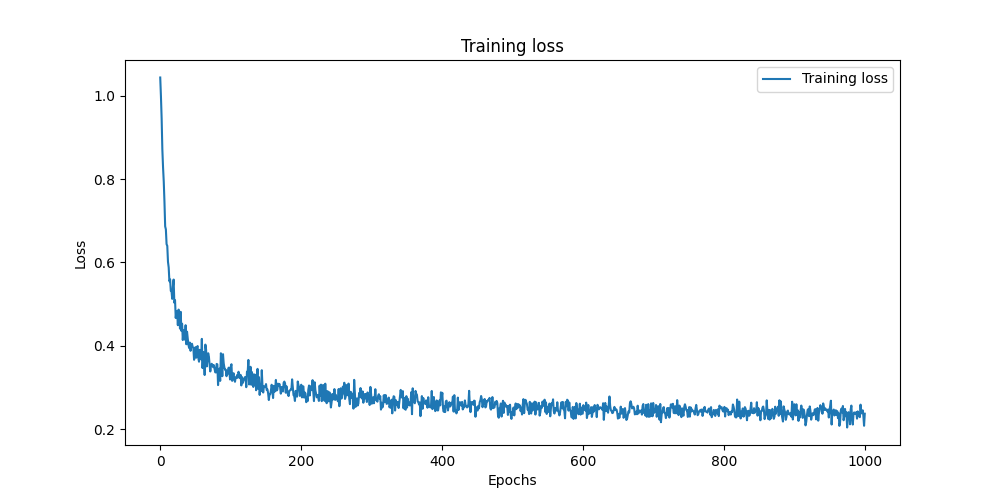
\includegraphics[width=0.7\textwidth]{plots/SASRec_ml-1m_training_loss.png}
    
    \caption{Training Loss for SASRec on MovieLens 1M}
    \label{fig:sasrec_loss}
\end{figure}

\begin{figure}
    \centering
    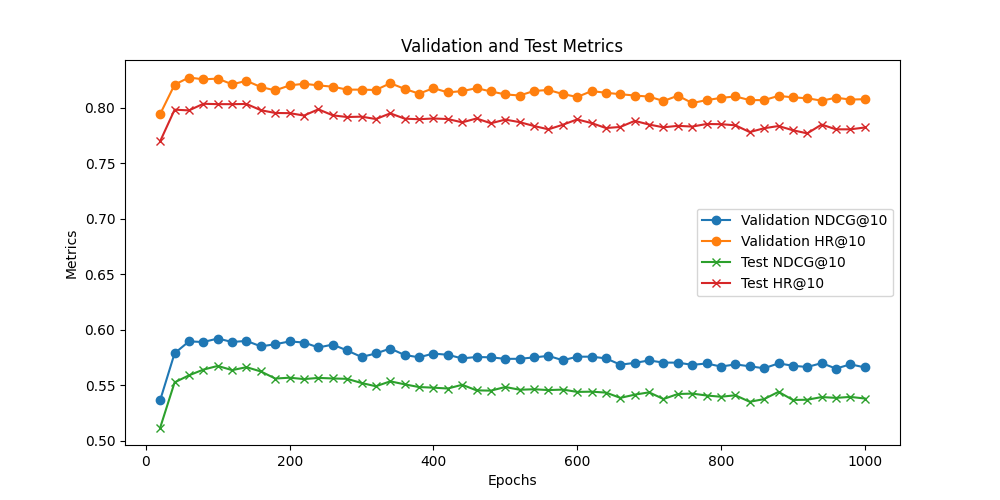
\includegraphics[width=0.7\linewidth]{plots/SASRec_ml-1m_metrics.png}
    \caption{HR@10 and NDCG@10) for SASRec on MovieLens 1M}
    \label{fig:enter-label}
\end{figure}


\begin{figure}[h!]
    \centering
    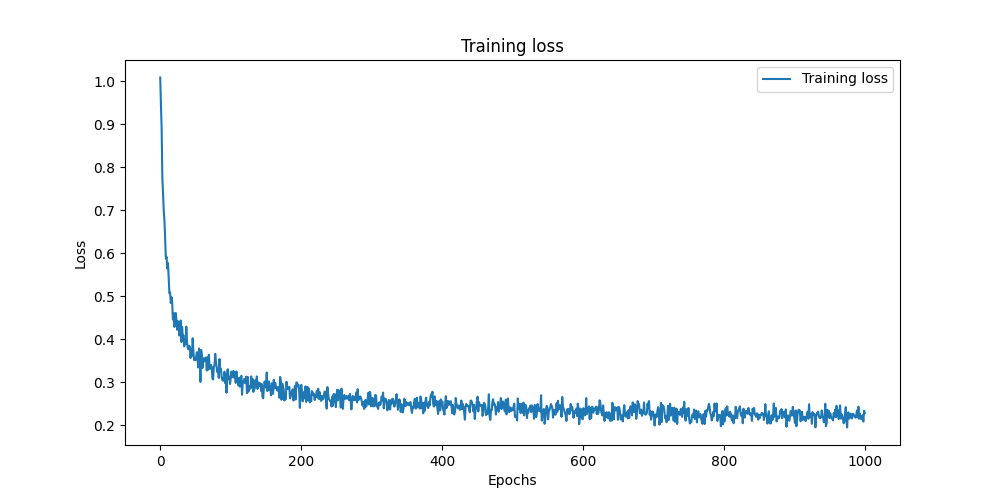
\includegraphics[width=0.7\textwidth]{plots/GRURec_ml-1m_training_loss.png}
    
    \caption{Training Loss for GRURec on MovieLens 1M}
    \label{fig:sasrec_loss}
\end{figure}

\begin{figure}
    \centering
    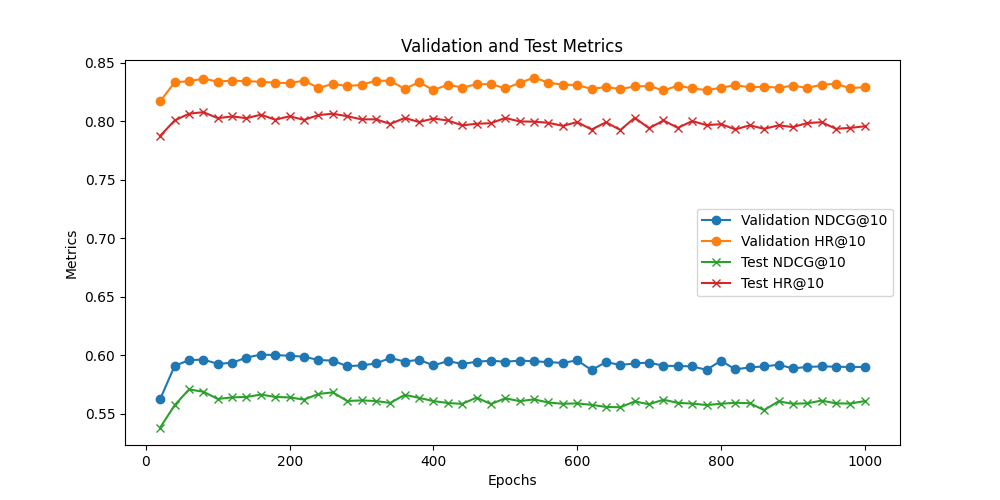
\includegraphics[width=0.7\linewidth]{plots/GRURec_ml-1m_metrics.png}
    \caption{HR@10 and NDCG@10) for GRURec on MovieLens 1M}
    \label{fig:enter-label}
\end{figure}


\begin{figure}[h!]
    \centering
    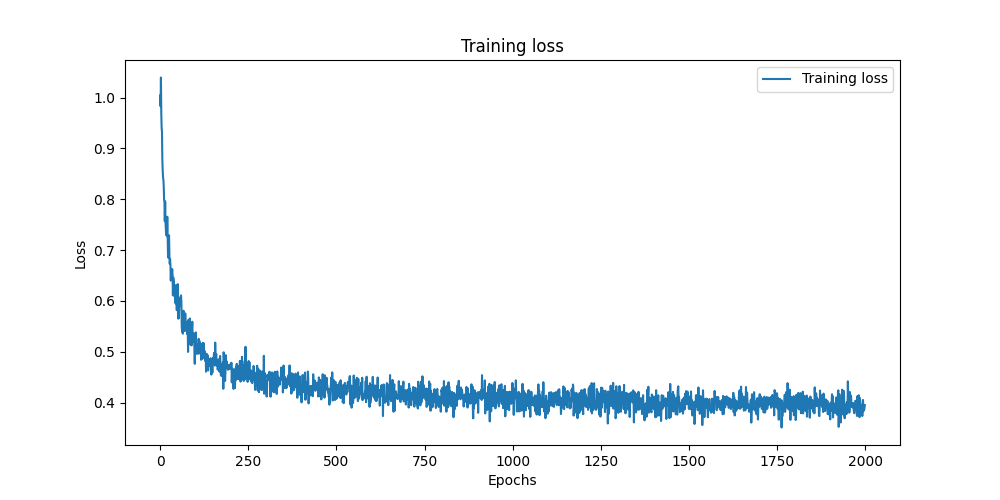
\includegraphics[width=0.7\textwidth]{plots/LMURec_ml-1m_training_loss.png}
    
    \caption{Training Loss for LMURec on MovieLens 1M}
    \label{fig:sasrec_loss}
\end{figure}

\begin{figure}
    \centering
    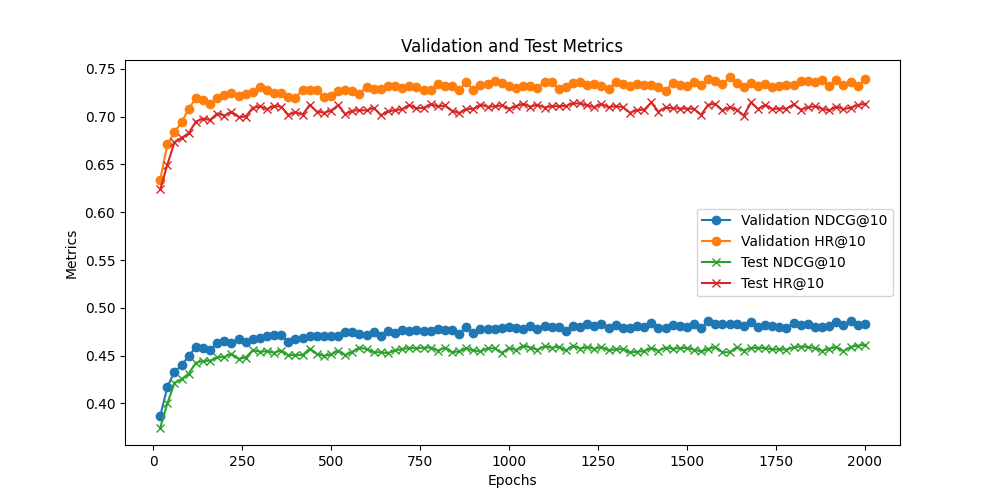
\includegraphics[width=0.7\linewidth]{plots/LMURec_ml-1m_metrics.png}
    \caption{HR@10 and NDCG@10) for LMURec on MovieLens 1M}
    \label{fig:enter-label}
\end{figure}


\section{Observations}

\begin{enumerate}
    \item \textbf{Performance of GRURec vs. SASRec:} Interestingly, GRURec outperformed SASRec in the initial iterations. However, after approximately 200 epochs, the performance of SASRec and GRURec converged, showing similar results. This indicates that GRURec demonstrated better performance during the early stages of training, but SASRec and GRURec achieved comparable performance in the later stages of training.

    \item \textbf{Performance of LMURec:} LMURec did not perform as well as expected. It was hypothesized that LMURec might perform better with longer sequence lengths. While this model did not excel with shorter sequences, its performance showed continuous improvement over time. This suggests that LMURec may be better suited for handling longer sequences, and further exploration with larger sequence lengths could be beneficial.

    \item \textbf{Sensitivity to Hyperparameters:} Experiments with different batch sizes and slight modifications in learning rates revealed that the MovieLens dataset is not highly sensitive to these parameters. This observation suggests that the choice of batch size and learning rate does not significantly affect the performance of the models on this dataset.
\end{enumerate}

\end{document}


